\section{Inleiding}

Nu machine learning steeds meer toepassingen krijgt, gaat men ook veel meer machine learning modellen gebruiken in de productieomgeving.
Traditioneel werden die modellen toegepast op centrale servers of gedistribueerde cloud servers. Hierdoor moet er een grote hoeveelheid data verstuurd worden over het internet.
Dat is echter niet zo schaalbaar als men op grote schaal met heel veel verschillende toestellen data gaat opmeten. % TODO: Waarom niet schaalbaar?

\begin{figure}[ht]
	\centering
	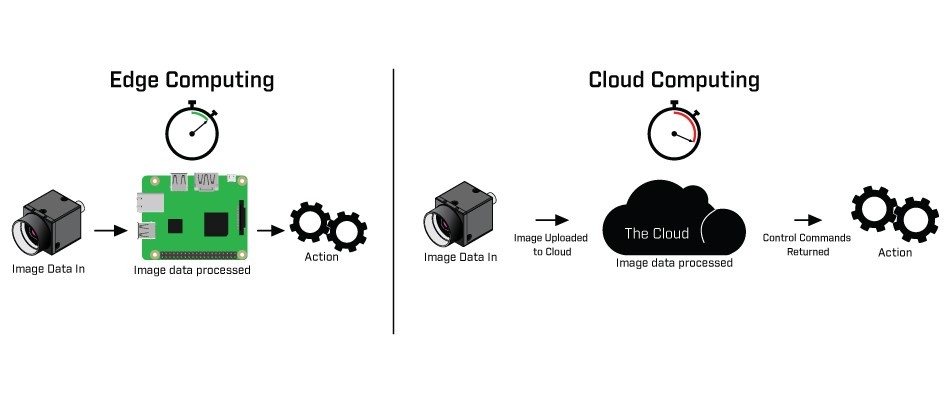
\includegraphics[width=0.9\textwidth]{figuren/iisedgecomputing.jpg}
	\caption{Edge vs. Cloud computing}
	\cite{flir-edge-computing}
	\label{fig:edge-vs-cloud}
\end{figure}

Er is gelukkig een grote 'paradigm shift' aan de gang waarbij men steeds meer machine learning gaat uitvoeren in embedded devices.
Dat is mogelijk omdat de embedded devices steeds sneller en beter worden in het verwerken van data.
Op die manier kunnen wij het machine learning model dichter bij de sensor plaatsen waardoor wij het benodigde netwerkverkeer minimaliseren.
Ook de latency of vertraging tussen opname en actie is veel kleiner. \cite{flir-edge-computing}

De ruwe data van de sensoren kan soms ook sensitieve informatie zoals gezichten of nummerplaten bevatten. Omdat we de data on-edge verwerken hoeven we die niet naar de cloud te sturen waar men ze kan onderscheppen. \cite{flir-edge-computing}
Het is echter niet zo simpel om de machine learning code, die geoptimaliseerd is voor multi-core servers, zomaar over te zetten naar de kleine, vaak single-core, microprocessors van die embedded devices.
% In dit verslag leg ik het proces om een machine learning model getraind in python, over te zetten naar C code voor een microcontroller.

\subsection{Doel van het project}

Het doel van dit project is met een Convolutional Neural Netwerk (CNN) geluidsevents te classificeren.
Die geluidsevents kunnen bijvoorbeeld spraak, een handenklap, gefluit of achtergrondgeluid zijn.
Dat is relatief simpel uit te voeren op een normale computer, maar het is dus niet praktisch om alle geluidsdata van meerdere meetpunten centraal te verwerken in real time.
Ook is het niet kost-effectief om overal aparte computers te plaatsen. In dit project gaan we dus het getraind CNN op een microcontroller uitvoeren om geluid van de ingebouwde microfoon te classificeren.

\section{Log-Mel feature extraction}

Het is mogelijk om een CNN te trainen op de onverwerkte geluidsdata.
Er zijn echter veel grotere modellen voor nodig, tot 34 lagen diep, en zal daarom ook sneller vatbaar voor overfitting. \cite{IEEE:very-deep-cnn-raw-waveforms}
Daarom is er toch een feature extraction stap gemaakt om de onverwerkte geluidsdata om te rekenen naar een Log-Mel-spectrogram.
Dit Log-Mel-spectrogram is eigenlijk een gewoon spectrogram waarvan we de frequentiebanden een beetje vervormd hebben zodat ze beter overeenkomen met de menselijke perceptie van geluid. \cite{enwiki:Mel-freq-cepstrum}

\begin{no-awa} % Zorgt ervoor dat de latex-2-awa parser deze environment negeert
De  Log-Mel feature extraction gebeurt in deze 5 stappen:

\begin{enumerate}
	\item DC-Normalisation
	      \begin{itemize}
		      \item Hiervoor gebruiken we een eerste orde IIR filter:
		            \begin{itemize}[label={}]
			            \item \(y\left[ n \right] = x\left[ n \right] - x\left[ n - 1 \right] -0.999 \cdot y\left[ n - 1 \right]\)
		            \end{itemize}
	      \end{itemize}

	\item Framing and windowing
	      \begin{itemize}
		      \item Eerst delen de audio op in frames van 32 ms die elk 10 ms overlappen met elkaar
		      \item Daarna passen we een Hamming-venster toe om hoogfrequente ruis te vermeiden \cite{enwiki:windowing}
	      \end{itemize}

	\item Discrete Fourier Transform (DFT)
	      \begin{itemize}
		      \item Met de DFT transformeren we elke frame van het tijdsdomein naar het frequentiedomein
		      \item We padden de frames totdat ze een macht van 2 zijn. Zo kunnen we het Fast Fourier Transform (FFT) algoritme gebruiken. Dit is sneller en accurater dan de normale DFT als er omdat er bij de gewone DFT meer afrondingsfouten kunnen gebeuren. \cite{enwiki:FFT}
		      \item Het resultaat is een vector met de magnitudes van elke frequentie in het signaal. Die vector is zeer hoogdimensionaal en is niet optimaal voor geluidsherkenning.
	      \end{itemize}

	\item Mel-frequency warping
	      \begin{itemize}
		      \item Mel-frequency warping transformeert de originele hoogdimensionale frequentievector naar een Mel-frequency vector. Zie Figuur~\ref{fig:Mel-bands}.
		            \begin{itemize}[label={}]
			            \item \(f_{Mel} = 2595\log_{10}(1 + \frac{f}{700})\)
		            \end{itemize}
		      \item Die Mel-frequency vector bevat minder frequentiebanden en is daardoor veel lager in dimensies. De Mel-banden zijn echter zo verspreid zodat ze veel beter overeenkomen met de menselijke perceptie van geluid.
	      \end{itemize}

	\item Feature normalisation and scaling
	      \begin{itemize}
		      \item Tenslotte normaliseren we de logaritmes van de Mel-magnitudes zodat het gemiddelde nul is, en de standaardafwijking één is:
		            \begin{itemize}[label={}]
			            \item \(m'_b = \frac{\ln\left( m_b \right) - \mu_b}{\sigma_b}\)
		            \end{itemize}
		      \item Als allerlaatste pre-processingstap gaan we de data schalen zodat die zich in het interval \(\left[ -1,1 \right]\) bevind. Zo kunnen ze opgeslagen worden in Q0.7 formaat. (Zie hoofdstuk~\ref{section:Qm.f} op pagina~\pageref{section:Qm.f})
	      \end{itemize}
\end{enumerate}
\end{no-awa}


\begin{figure}[ht]
	\centering
	\includegraphics[width=0.6\textwidth]{figuren/Mel-frequency.png}
	\caption{Mel-frequency warping}
	\cite{efficient-feature-extraction}
	\label{fig:Mel-bands}
\end{figure}


\section{Convolutional Neural Network (CNN)}

Om met de Log-Mel samples geluidsevents te kunnen herkennen, gebruik ik een Convolutional Neural Network (CNN). Ons model bestaat uit meerdere verschillende lagen. De belangrijkste lagen zijn de convolutielagen. De eerste convolutielaag past een 2D-convolutie toe op het Log-Mel-spectrum met een bepaald aantal filters. Die filters gaan we optimaliseren met machine learning.
Na elke convolutielaag voegen we een ReLU activation laag toe. (niet weergegeven op figuur~\ref{fig:cnn-model}) De ReLU activatiefunctie is snel en gemakkelijk te berekenen, \cite{enwiki:relu} maar kan soms lijden tot een 'vanishing gradient'. \cite{enwiki:vanishing-gradient}

Om de dimensionaliteit van onze lagen kleiner te maken, introduceren wij een max pooling laag na elke activatielaag. Die laag neemt het maximum van een aantal waardes en laat de rest vallen. Daarna plaatsen wij een dropout laag. (niet weergegeven op figuur~\ref{fig:cnn-model}) Die gaat willekeurig, met een kans van 50 \%, de resultaten van verschillende convolutiefilters met nul vermenigvuldigen en dus laten vallen. Dit is om overfitting tijdens het trainen tegen te gaan.

\begin{figure}[ht]
	\centering
	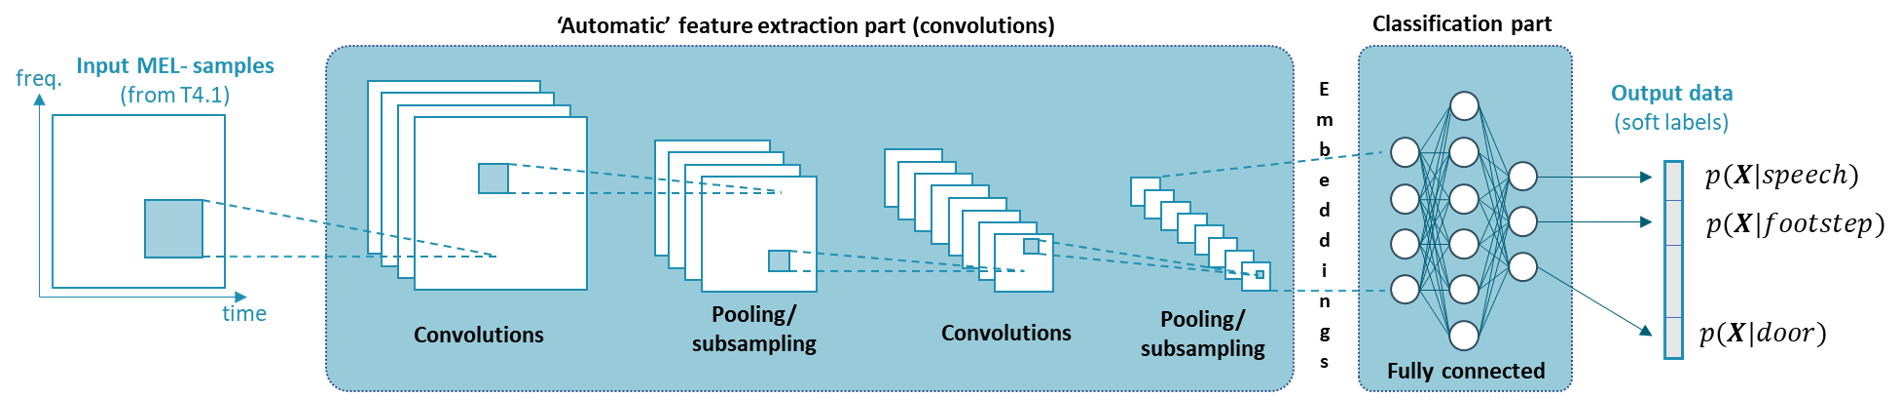
\includegraphics[width=0.9\textwidth]{figuren/cnn.png}
	\caption{Voorbeeld van een CNN model}w
	\cite{slides:cnn}
	\label{fig:cnn-model}
\end{figure}

Die vier lagen (convolutie, activatie, max pooling en dropout) herhalen we drie keer. Daarna schakelen we over naar een traditioneel neuraal netwerk, ookwel 'fully connected netwerk' genoemd. Die bestaat uit fully connected layers of perceptronlagen, activatielagen en dropout lagen. Als allerlaatste outputlaag gebruiken wij een softmax activation layer om een genormaliseerde kansverdeling over de verschillende geluidsklassen. \cite{enwiki:softmax}

% TODO: Maybe add a table with the specific structure of the model and the amount of parameters

\subsection{Trainen van het model}
\subsubsection{Installatie Python en Tensorflow}
Het trainen van het model hebben we gewoon gedaan op onze computers in python. Hiervoor hebben wij de Keras uit de TensorFlow package gebruikt. Het installeren van alle benodigde packages ging echter niet vlekkeloos. Uit de TensorFlow documentatie konden we afleiden dat we specifiek Python 3.8 moesten installeren in plaats van de meest up-to-date versie van python. Dan bleek dat er nog meer packages nodig waren. Toch kon ik het relatief snel alle problemen oplossen.

% TODO: Decide if I leave this paragraph in or not
Voor Python gebruik ik Visual Studio Code, een all round text editor, om de code te schrijven en Powershell, een command line interface, om mijn Python omgeving manueel te managen. Ik vermoed dat ik, door die ervaring met Python projecten handmatig op te starten, gemakkelijker alle installatieproblemen kon vinden en oplossen.
Een requirements.txt file \cite{pip-user-guide} had bijvoorbeeld al een goede hulp geweest voor het installeren van de juiste packages.

\subsubsection{Resultaten}
Ik heb mijn model 400 epochs getrained in plaats van 250. Ik was namelijk vroeg klaar met al de rest en heb zo dus wat extra getained om te kunnen vergelijken. Omdat de model loss lager is bij 400 epochs dan bij 250 epochs, kunnen we afleiden dat het model waarschijnlijk beter is na 400 epochs. (zie figuur~\ref{fig:cnn-training})

\begin{figure}[ht]
	\centering
	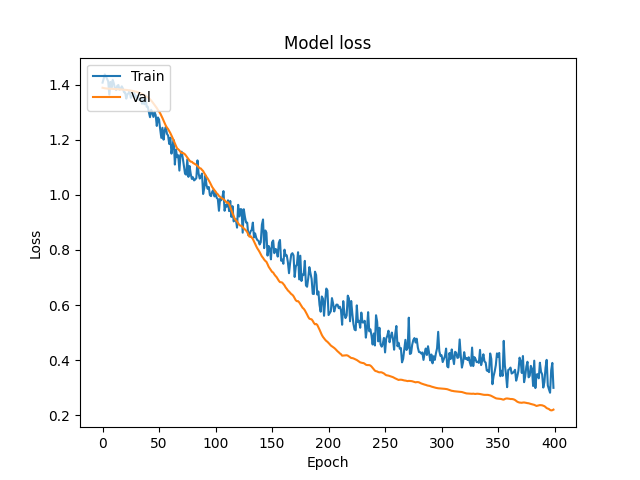
\includegraphics[width=0.7\textwidth]{figuren/cnn_model.png}
	\caption{Loss van het model per epoch}
	\label{fig:cnn-training}
\end{figure}

\newpage

% TODO: Talk about F1 Score and such
In de confusion matrix (tabel~\ref{tab:confusion-matrix}) kunnen we zien dat het model het moeilijkste spraak kan detecteren.
Ik vermoed dat dat is omdat spraak het meest complexe spectrum zal geven. Achtergrondgeluid zal waarschijnlijk gewoon zacht geluid zijn, handgeklap is een luide impuls en fluiten is een relatief zuivere constante toon. Omdat het grootste deel correct wordt herkent, denk ik dat mijn model goed werkt. Ook uit de classification report van scikit-learn (tabel~\ref{tab:classification-report}) kunnen we zien dat mijn model zeer goed werkt.
Per metric zijn de macro average en weighted average hetzelfde omdat de elke klasse even vaak voorkomt. De validatieset is dus helemaal gelijk verdeeld.

\begin{table}[ht]
	\centering
	\begin{tabular}{ |c|c|c|c|c||c| }
		\cline{2-6}
		\multicolumn{1}{c| }{} & Predicted: & Predicted: & Predicted: & Predicted: &       \\
		\multicolumn{1}{c| }{} & background & handclap   & speech     & whistle    & Total \\

		\hline Actual:         &            &            &            &            &       \\
		background             & 25         & 0          & 0          & 0          & 25    \\

		\hline Actual:         &            &            &            &            &       \\
		handclap               & 1          & 23         & 1          & 0          & 25    \\

		\hline Actual:         &            &            &            &            &       \\
		speech                 & 0          & 3          & 22         & 0          & 25    \\

		\hline Actual:         &            &            &            &            &       \\
		whistle                & 0          & 0          & 0          & 25         & 25    \\
		\hline\hline
		                       &            &            &            &            &       \\
		Total                  & 26         & 26         & 23         & 25         & 100   \\
		\hline
	\end{tabular}
	\caption{Confusion matrix}
	\label{tab:confusion-matrix}
\end{table}

\begin{table}[ht]
	\centering
	\begin{tabular}{ |l|r|r|r|r| }
		\cline{2-5}
		\multicolumn{1}{c| }{} & Precision & Recall & \( F_1 \)-score & Support \\
		\hline
		Background             & 0.96      & 1.00   & 0.98            & 25      \\
		Handclap               & 0.88      & 0.92   & 0.90            & 25      \\
		Speech                 & 0.96      & 0.88   & 0.92            & 25      \\
		Whistle                & 1.00      & 1.00   & 1.00            & 25      \\

		\hline\hline
		Accuracy               &           &        & 0.95            & 100     \\
		Macro average          & 0.95      & 0.95   & 0.95            & 100     \\
		Weighted average       & 0.95      & 0.95   & 0.95            & 100     \\
		\hline
	\end{tabular}
	\caption{scikit-learn Classification Report van het model}
	\label{tab:classification-report}
\end{table}

\section{Edge implementatie}
We hebben nu een goed getraind model op onze computer staan. Dit model moeten we nu opnieuw implementeren in C code om heel performant te werken op onze microcontroller. Zo kunnen we in real-time geluid opnemen met de ingebouwde microfoon en zo classificeren als achtergrondgeluid, een handenklap, spraak en gefluit. Dit blijkt echter niet zo simpel te zijn.

\subsection{Kwantisatie van ons CNN-model}
In python gebruikt het model floating point getallen. Floating-point getallen zijn zeer flexibel met een hoge 'dynamic range', wat goed is om te trainen, maar niet het meest performant of nauwkeurig voor grote getallen. Dit komt omdat het getal en de positie van de comma als aparte delen in één getal worden opgeslagen. \cite{enwiki:floating-point} We gaan die dus flexibiliteit opofferen door over te schakelen naar fixed-point getallen. Dit kunnen we ook doen omdat de gewichten nu vast bepaald zijn na het trainen.

\subsubsection{Qm.f formaat}
\label{section:Qm.f}
% TODO: Explain Qm.f format

\subsubsection{Exporteren van gewichten}
Om de gewichten van onze modellen te exporteren, gebruiken we het k2arm.py script. Dit script gaat automatisch alle weights en biases omvormen van floating point nummers tot fixed-point nummers van 8 bits, waarvan één tekenbit. Zo nemen ze zeer weinig plaats in in het geheugen van de microcontroller. Hierbij zal hij voor elke laag de positie van de comma op voorhand bepalen.

\subsection{Experiment met microfoon}
\subsubsection{Resultaten}


\section{Conclusie}